% Author: Till Tantau
% Source: The PGF/TikZ manual

\documentclass{article}

\usepackage{pgf}
\usepackage{tikz}
\usetikzlibrary{arrows,automata}
\usepackage[latin1]{inputenc}
\usepackage{verbatim}

\begin{document}

\begin{comment}
:Title: State machine
:Tags: Manual, Automata, Graphs

Another examle from the manual.

| Author: Till Tantau
| Source: The PGF/TikZ manual

\end{comment}

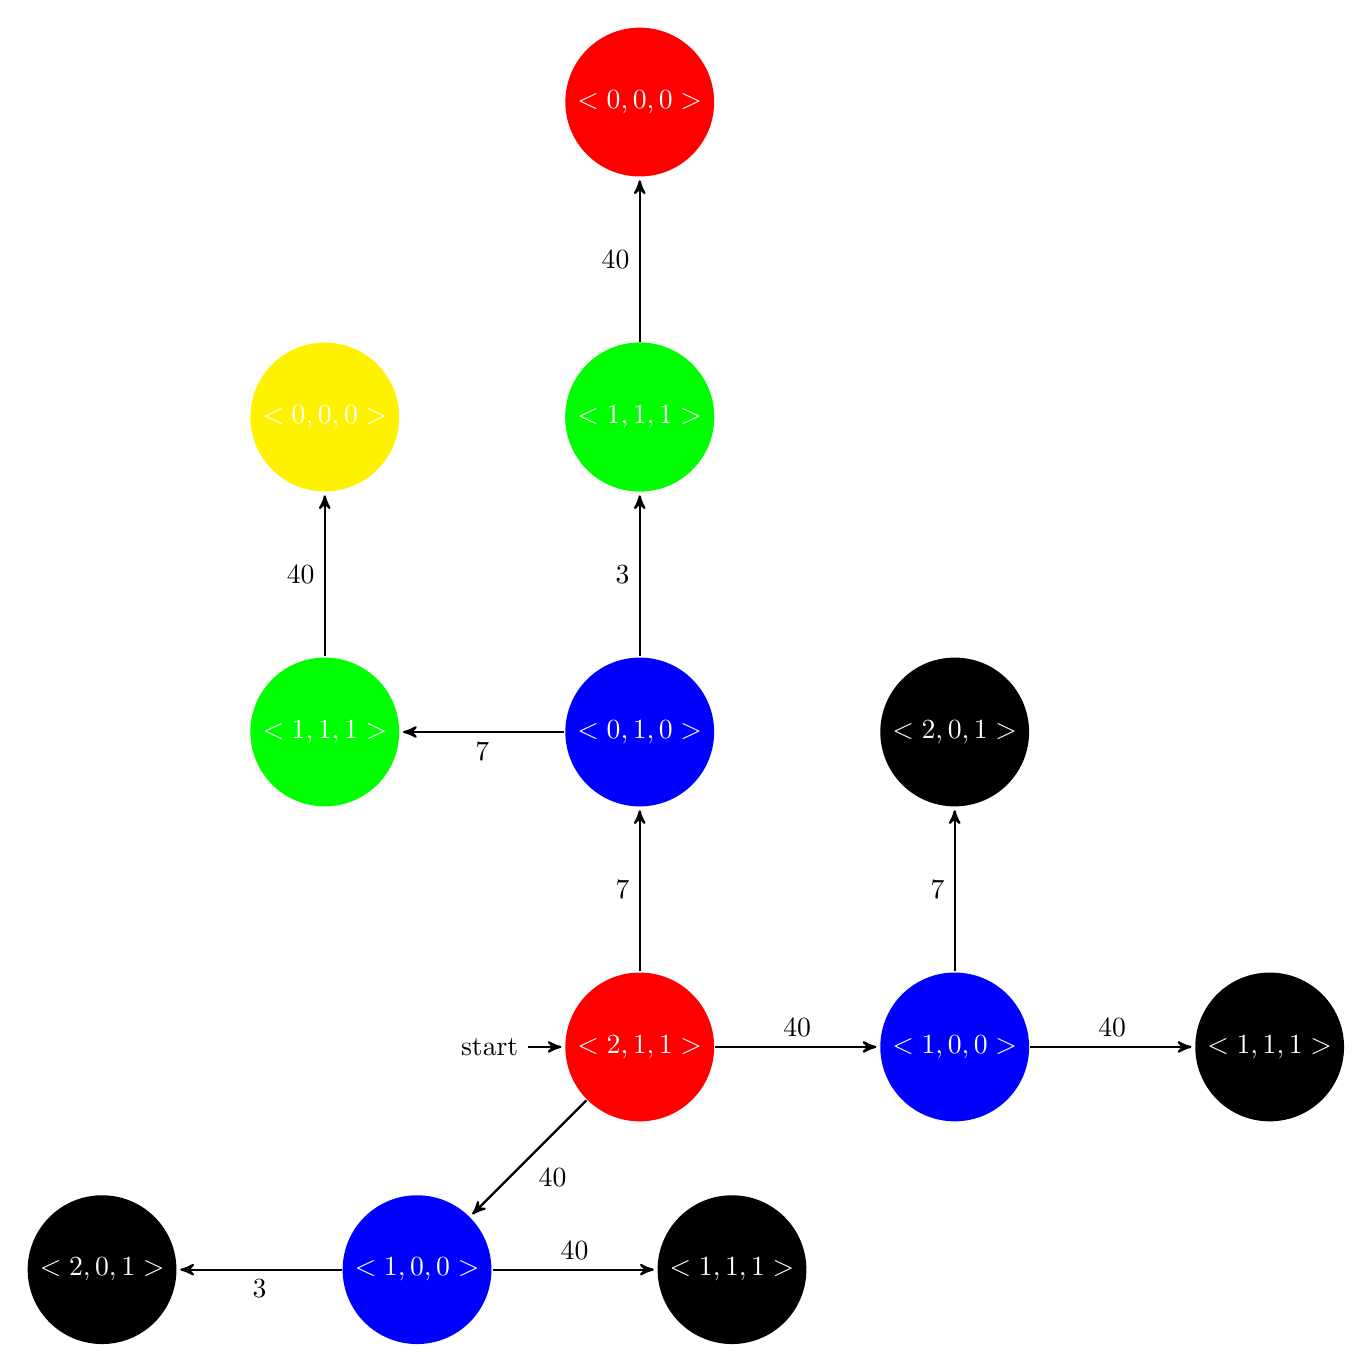
\begin{tikzpicture}[->,>=stealth',shorten >=1pt,auto,node distance=4.0cm,
                    thick]
  \tikzstyle{every state}=[fill=red,draw=none,text=white]

  \node[initial,state] (A)                    				{$<2,1,1>$}; % Inicial
  \node[state,fill=blue]         (B) [above of=A] 	  		{$<0,1,0>$}; % 2 ARQ
  \node[state,fill=blue]         (C) [right of=A]       	{$<1,0,0>$}; % 1 1
  \node[state,fill=blue]         (D) [below left of=A] 		{$<1,0,0>$}; % 1 1
  \node[state,fill=green]		 (E) [above of=B]			{$<1,1,1>$}; % 1 1 
  \node[state,fill=green]		 (F) [left of=B]			{$<1,1,1>$}; % 1 1
  \node[state,fill=black]		 (G) [above of=C]			{$<2,0,1>$};
  \node[state,fill=black]		 (H) [right of=C]			{$<1,1,1>$};
  \node[state,fill=black]		 (I) [left of=D]			{$<2,0,1>$};
  \node[state,fill=black]		 (J) [right of=D]			{$<1,1,1>$};
  \node[state,fill=green]		 (K) [above of=B]  			{$<1,1,1>$};
  \node[state,fill=yellow] 		 (L) [above of=F] 			{$<0,0,0>$};
  \node[state,fill=red] 		 (M) [above of=K] 			{$<0,0,0>$};
  \path (A) edge              	node {7}   (B)
        (A) edge              	node {40}  (C)
        (A) edge              	node {40}  (D)
        (B) edge			  	node {3}   (E)
        (B) edge			  	node {7}   (F)
        (C) edge				node {7}   (G)
        (C) edge				node {40}  (H)
        (D) edge				node {3}   (I)
        (D) edge				node {40}  (J)
        (E) edge				node {40}  (M)
        (F) edge				node {40}  (L)
       ;
\end{tikzpicture}

\end{document}


% 2 Arqueologos y 1 Canibal
% Velocidades 5,10 ARQ , 15 Canibal
%
%Tenemos 2 Arqueologs y 1 Canibal

% Velocidades 3 , 7 y 40


% El algoritmo empieza en el nodo rojo central
% y encola los 3 nodos azules,mira primero
% el que esta justo arriba (se mandaron los 2 arqueologos).pues es el que tiene menor costo.

% Como no es el nodo que buscamos encolamos los 2 verdes
% que tienen costo total de 10 y 14 respectivamente.
% Como sus costos son menores a 40 lo miramos primero
% y como no son el objetivo, encolamos sus hijos
% amarillos/rojo que son una solucion posible.

% Ahora miramos los 2 nodos azules del principio. como no son el buscado
% se encola a sus hijos.

% Finalmente agarramos el otro nodo rojo, como es el estado buscado devolvemo
% su costo total